
\section{Stencils, Borders and Partitioned Arrays}
\label{sec:Stencils}

\begin{figure}
\[	\stencil{Sobel_X}{rrr}
	{ -1 &  0 & +1 \\
	  -2 &  0 & +2 \\
	  -1 &  0 & +1 } \\
%
	\stencil{Roberts_X}{rr}
	{ +1 &  0 \\
	   0 & -1 }
%
	\stencil{Kirsch_W}{rrr}
	{  5 & -3 & -3 \\
	   5 &  0 & -3 \\
	   5 & -3 & -3 }
\]
\[	\stencil{PeakPoint}{rrr}
	{  -1 & -1 & -1 \\
	   -1 & 8  & -1 \\
	   -1 & -1 & -1 }
%
	\stencil{HighPass}{rrrrr}
	{  0 &   1 &  -1 &   1 &   0 \\
	   1 &  -2 &   4 &  -2 &   1 \\
	   1 &   4 & -13 &   4 &   1 \\
	   1 &  -2 &   4 &  -2 &   1 \\
	   0 &   1 &  -1 &   1 &   0 }
\]
\[	\stencil{Binomial_{7X}}{rrrrrrr}
	{ 1 & 6 & 15 & 20 & 15 & 6 & 1 }
%
	\stencil{Laplace}{rrr}
	{ 0 & 1 & 0 \\
	  1 & 0 & 1 \\
	  0 & 1 & 0 }
\]
\caption{Common convolution stencils}
\label{Fig:ExampleKernels}
\end{figure}

Several common stencils are shown in Figure \ref{Fig:ExampleKernels}. For stencil names written with subscripts, the subscript indicates that it is just one member of a closely related family of stencils. For example, $Sobel_X$ differentiates along the X axis only, but rotating it 90 degrees yields $Sobel_Y$ which differentiates along the Y axis. By ``rotate'' we mean to permute the coefficients of the matrix, so that +1 is in the top-left in this example. The $Sobel_{X,Y}$ stencils are used in Canny edge detection, while $Roberts_X$ and $Kirsch_W$ also perform discrete differentiation. The $PeakPoint$ stencil is used for noise detection, $HighPass$ is a high-pass filter, and $Binomial_{7X}$ is a low-pass filter. The $Laplace$ stencil is used to compute the average of four surrounding pixels, which we discussed in \S\ref{sec:Laplace}. How these stencils are derived is not important to the discussion, but see \cite{O'Gorman:algorithms-for-image-analysis} for a nice introduction to stencil convolution and other image processing algorithms. For the example stencils, we note several features of computational interest, along with exceptions: 

\begin{enumerate}
\item	All coefficients are statically known.
\item	Most coefficients are small integers.
\item	Many coefficients are zero.
\item	All stencils are symmetric. 
\item	All stencils contain repeated coefficients.
\item	Most stencils fit in a 5x5 matrix.
\item	Most stencils are square. (except $Binomial_{7X}$)
\item	Most stencils have odd dimensions. (except $Roberts_X$)
\end{enumerate}

Points 1 and 2 suggest that we can specialise our stencil functions based on the values of the coefficients. For example, multiplication by two can be achieved by addition, and multiplication by one is no-op. This is opposed to, say, writing a general purpose function that reads coefficients from an array, and performs all multiplications explicitly. Points 3, 4 and 5 suggest that there are savings to be had by common sub-expression and dead-code elimination. Point 6 suggests that being able to handle stencils smaller than a certain fixed size would allow us to support most of the common cases. Points 7 and 8 have implications for border handling, which we discuss in the next section. 


% -----------------------------------------------------------------------------
\subsection{Partitioned Arrays}
\label{sec:PartitionedArrays}
\label{sec:BordersAndPartitionedArrays}


% ------------------------------------- FIG
\begin{figure}
\begin{center}
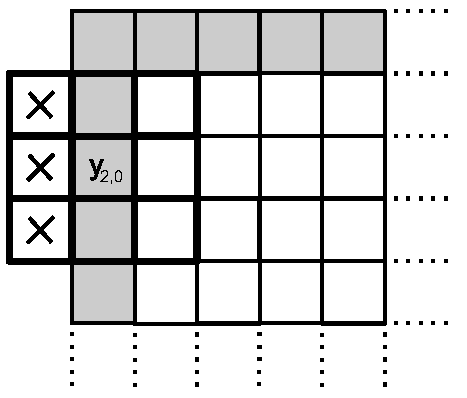
\includegraphics[scale=0.5]{figs/StencilBorder.eps}
\end{center}
\caption{Application of a 3x3 stencil in the border region}
\label{fig:StencilBorder}
\end{figure}

When implementing convolution, an immediate concern is what to do when the stencil ``falls off'' the edge of the array. For example, Figure \ref{fig:StencilBorder} shows the application of a 3x3 stencil in this circumstance. The white squares indicate the \emph{internal} region, where the stencil is entirely within the array. The grey squares indicate the \emph{border}, where part of the stencil falls outside. There are several ways of handling the border case, with two popular options being to return a constant value (like zero) for out-of-bounds elements, or to return the same value as the nearest in-bounds element. 

With the array sizes commonly encountered during image processing, only a tiny fraction of the elements are in the border region. This fact implies that for optimal performance, we should avoid testing for the border each time we compute an element. To achieve this, we represent the \emph{partitioning} of the array into various regions directly. Partitioning allows us to define the result array using element functions specialised to each region, and guarantee that the one producing the internal elements is not applied in the border region. In effect, partitioning the array allows us to lift the \textbf{if}-expression that tests for the border out of the main loop of our program, and have the library code construct the border and internal regions separately. With partitioned arrays, it does not matter if the element function for the border takes a little longer to evaluate than the one for the internal region, as the former is only applied a small number of times. Provided the simpler, internal case is well optimised, we will still get good overall performance. 


% ------------------------------------- FIG
\begin{figure}
\begin{small}
\begin{code}
data Array sh a
   = Array       { arrayExtent  :: sh
                 , arrayRegions :: [Region sh a] }
data Region sh a
   = Region      { regionRange  :: Range sh
                 , regionGen    :: Generator sh a }
data Range sh 
   = RangeAll
   | RangeRects  { rangeMatch   :: sh -> Bool
                 , rangeRects   :: [Rect sh] }
data Rect sh
   = Rect sh sh

data Generator sh a
   = GenManifest { genVector   :: Vector a }	
	
   | forall cursor. 
     GenCursored { genMake     :: sh -> cursor
                 , genShift    :: sh -> cursor -> cursor
                 , genLoad     :: cursor -> a }
\end{code}
\end{small}
\caption{New Repa array types}
\label{fig:NewRepaArrays}
\end{figure}


Our new data types are shown in Figure \ref{fig:NewRepaArrays}. An @Array@ is defined as an extent, and a list of distinct @Regions@. In the rank-2 (two-dimensional) case the extent will represent the width and height of the array. Each region has a @Range@ that defines the set of indices belonging to the region. A @Range@ can either be @RangeAll@, which indicates the entire array, or a @RangeRects@ which gives a list of rectangles (of arbitrary rank). Given a @RangeRects@, we can determine whether a particular index is inside the range either by checking whether it falls in any of the @Rects@, or using the predicate @rangeMatch@. This predicate gives the same result as the former, but can use a more efficient implementation than checking each @Rect@ individually. In general, for ``local'' array operations such as indexing a single element, we use the predicate to quickly determine which region the provided index is in. In contrast, @rangeRects@ is used when forcing the entire array, and allows us to create a loop specialised to each region. 

Each @Region@ also has a @Generator@ that encodes how the array elements in that region should be computed. As before, generators of @Manifest@ arrays are just flat vectors of unboxed values that hold the elements in row-major order. Delayed arrays are now represented in \emph{cursored} form. The cursored representation allows us to share indexing computations when forcing adjacent array elements, which is discussed further in \S\ref{sec:SharingAndCursoredArrays}. The regions of a partitioned array must provide \emph{full coverage}, meaning that every array element must be within some region. Regions are permitted to overlap, with the first one in the list taking precedence. Using overlapping allows us to define a default value for array elements with a @RangeAll@, while carving out specific areas with a @RangeRects@ earlier in the list.
 
In general, partitioning an array allows us to generate loops specialised to each region. Specialisation can occur on both a per-element and per-region basis. An example of the first is the optimisation of border handling, which we discussed earlier. An example of the second is to use different loop code to evaluate regions of different sizes. For example, when evaluating a region that is short and wide it is best to operate in a row-wise manner, computing an entire row before moving to the next. This helps to recover sharing between horizontally adjacent elements. In contrast, to evaluate a region that is tall but thin it is best to operate column-wise, to exploit sharing between vertically adjacent elements. As the @Region@ type provides a direct description of the size of each region, we can specialise the library code based on this information. The user invokes the appropriate specialisation automagically with each application of @force@. We discuss specialisation further in \S\ref{sec:FillingTheArray}.


% -----------------------------------------------------------------------------
\subsection{Bounds Checking and co-Stencils}
\label{sec:CoStencils}
Firstly, with respect to bounds checking, we sheepishly admit that the old version of Repa didn't actually do any. This issue was mentioned in \cite{Keller:repa}. As such, it was possible for buggy client programs to crash at runtime. The trouble is that bounds checking each array access adds a substantial overhead, and the comparison and branching constructs involved interfere with fusion. We tried adding it, by having the @Data.Vector@ library check each of the indexing operations on the underlying manifest array, but this resulted in a 35\% slowdown for our Laplace example applied to a 300x300 array. 

Ultimately, the problem is that client code written by the user of a library is ``untrusted'', meaning that the library must assume it will index out-of-bounds elements. With respect to the code in Figure \ref{fig:LaplaceIndex}, without a more ``heavy weight'' technology like dependent types, or some clever analysis, the compiler cannot prove that when the predicate @isBorder@ succeeds, the indexing operations in the @else@ branch of @elemFn@ are guaranteed to be valid. This problem is compounded by the fact that to support shape polymorphism we must check indices of arbitrary rank against the array bounds. Failing that we could check the linear indexing of the underlying manifest vector, but we would still need to manage the mapping between these indices and the original indices of arbitrary rank.

Our solution to this problem is to invert the relationship between the stencil definition (@elemFn@) and the source array. Instead of having the (untrusted) @elemFn@ fetch elements from the source array itself, we instead write the client code to combine source elements fed to it by the (trusted) library. This distinction is similar to the one between recursive and co-recursive functions in stream fusion \cite{Coutts:stream-fusion}, where the latter is the ``co-stencil'' case. Related work on Ypnos \cite{Orchard:ypnos} mentions the co-monadic structure of grid computations, but does not discuss the relationship with bounds checking. 

Figure \ref{fig:Stencils} gives the data type that represents stencils, while Figure \ref{fig:NewSolveLaplace} contains our new implementation of @solveLaplace@. Figure \ref{fig:Stencils} also gives the definition of @makeStencil@ which is a utility function defined by our library. The type @Stencil sh a@ specifies a stencil function of shape @sh@ that operates on arrays of element type @a@. It consists of a size such as @Z:.3:.3@ for the 3x3 case, as well as a zero value and accumulator function which define a fold operation over array elements. Figure \ref{fig:NewSolveLaplace} shows how to define the Laplace stencil. The @iterateBlockwise@ function repeatedly applies its parameter function to an array, forcing it after each iteration. In this and latter code we have elided @INLINE@ pragmas, as well as the @Shape@ and @Elt@ type class constraints to save space. We have also elided explicit matches against the input arrays @arrBoundMask@, @arrBoundValue@ and @arrInit@ that require them to be manifest. These matches are needed in our concrete implementation for performance reasons, but we hope to improve the compiler so they are not required in future. This is discussed further in \S\ref{sec:MultiStage}. 

The lambda abstraction in the definition of @laplace@ defines the \emph{coefficient function} for the Laplace stencil. The coefficient function gives the coefficients for each position in the stencil, and has type @(sh -> Maybe a)@. It gives the coefficient at a particular offset from the \emph{focus} of the stencil, or if that coefficient is zero it returns @Nothing@ instead. Handling of zeros is discussed further in the next section. As a syntactic convenience, our library also provides some Template Haskell code to make listing the coefficients easier. An example of this syntax is in the @niceLaplace@ function of  Figure \ref{fig:NewSolveLaplace}.
 
The operation of computing the sum-of-products of array elements and stencil coefficients is defined by the @Just@ case of @makeStencil@. We could have embedded the coefficient function directly in the definition of @Stencil@, but instead define stencils in terms of a more general fold operation. Using a fold leaves the door open for other stencil-like operations that are not expressed as a sum-of-products, such as the creation of a histogram of the neighbourhood of each pixel.

Returning to the issue of bounds checking, with our new definitions, client code does not need direct access to the source array at all. All of the library functions used in Figure \ref{fig:NewSolveLaplace} operate on the whole array at a time, and their safety depends on the correctness of the library, instead of the correctness of the client.

Finally, we note that in virtually all related work using imperative languages it is simply assumed that bounds checking is not performed. The focus of recent papers such as \cite{Datta:stencil-computation-autotuning} and \cite{Krishnamoorthy:auto-paralellization-of-stencils} is usually on optimising cache usage, and they presume the existence of correct, heavily optimised straight line code for computing the individual array elements. In contrast, we are trying to produce a (safe!) general purpose functional array library, which also has support for efficient stencil convolution. 

% ----------------- FIG
\begin{figure}
\begin{small}
\begin{code}
data Stencil sh a
   = Stencil { stencilSize  :: sh 
             , stencilZero  :: a
             , stencilAcc   :: sh -> a -> a -> a }

makeStencil :: sh -> (sh -> Maybe a) -> Stencil sh a
makeStencil ex getCoeff
 = Stencil ex 0 
 $ \ix val acc
    -> case getCoeff ix of
          Nothing     -> acc
          Just coeff  -> acc + val * coeff
\end{code}
\end{small}
\caption{Stencils and stencil construction}
\label{fig:Stencils}
\end{figure}


% ----------------- FIG
\begin{figure}
\begin{small}
\begin{code}
solveLaplace :: Int -> Image -> Image -> Image -> Image
solveLaplace steps arrBoundMask arrBoundValue arrInit
 = iterateBlockwise steps arrInit
 $ zipWith (+) arrBoundValue 
 . zipWith (*) arrBoundMask
 . map (/ 4) . mapStencil2 (BoundConst 0) laplace

laplace :: Stencil sh a
laplace     =  makeStencil (Z :. 3 :. 3)
            $ \ix -> case ix of
                      Z :.  0 :.  1 -> Just 1
                      Z :.  0 :. -1 -> Just 1
                      Z :.  1 :.  0 -> Just 1
                      Z :. -1 :.  0 -> Just 1
                      _             -> Nothing

niceLaplace :: Stencil sh a
niceLaplace =  [stencil2| 0 1 0
                          1 0 1 
                          0 1 0 |]
\end{code}
\end{small}	
\caption{Stencil based Laplace function}
\label{fig:NewSolveLaplace}
\end{figure}


% -----------------------------------------------------------------------------
\subsection{Zeros in Stencil Definitions}
Although the stencils we use often contain zero-valued coefficients, we want to avoid wasting cycles performing the corresponding multiplications, as they do not contribute to the final sum of products. The simple, neat and \emph{wrong} solution is to allow terms of the form $0*x$ in the intermediate code, but then add a GHC rewrite rule \cite{PeytonJones:playing-by-the-rules} to implement the obvious identities $0*x \equiv 0$ and $x+0 \equiv x$. Unfortunately, the first one of these is invalid for standard \mbox{IEEE-704} floating point numbers because the operation $0*\infty$ is supposed to produce NaN (Not a Number). Although this hardly matters for image processing, we still don't want to add the rule as it would apply globally and we risk breaking other code. Instead, we define the coefficient function to return @Nothing@ where the stencil does not apply, and use this to skip over the associated term in @makeStencil@. Nevertheless, in the literature, stencils are usually specified using zeros. Due to this we allow zeros in our Template Haskell version, but eliminate them while desugaring to the coefficient function. 

